\documentclass[a4paper,11pt]{article}
\usepackage[utf8]{inputenc}
\usepackage{dmasproject}
% if you need additional LaTeX packages, add them here
\usepackage[T1]{fontenc}
\usepackage{newpxtext,newpxmath}
% \usepackage[left=1in, right=1in, top=1.25in, bottom=1.25in]{geometry}
\usepackage{hyperref}
\usepackage{titling}

% \usepackage{caption}
\usepackage{amsmath}
\usepackage{mathtools}
\usepackage{amsfonts}
\usepackage{amssymb}
\label{mathrefs}

\usepackage{graphicx}
\usepackage{multirow}
\usepackage{pdflscape}

% Remove paragraph indent and add space between paragraphs
\usepackage{parskip}
\setlength{\parindent}{0pt}

% \hypersetup{
%     colorlinks=true,
%     linkcolor=blue
% }

\begin{document}

% Ask zain and connor to review safety/regulatory section and update
% Waleed help with proj management (sec 9)

%% BEGIN TITLE
\begin{titlingpage}
    \begin{center}
        {\huge\bfseries%
            University of Waterloo \\
        }
        \vspace{1em}
        {\Large\bfseries%
            Faculty of Engineering \\
            \vspace{1em}
            GENE 404 Design Project Report \\
        }
        
        \vspace{10em}
    
        % Heading
        \begin{figure}[H]
            \centering
            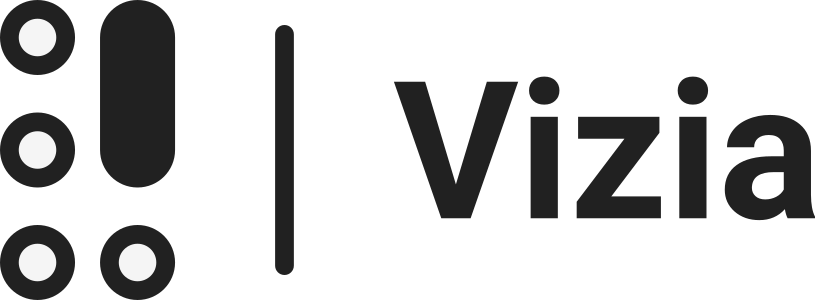
\includegraphics[scale=0.45]{img/logo_text_dark.png}
        \end{figure}
        {\Huge\bfseries%
            Glasses for the Visually Impaired \\[0.5em]
        }

        \vspace{10em}
        
        % Authors
        Prepared by: \\
        \vspace{1em}
        \begin{tabular}{cccc}
            Waleed Ahmed & Martin Ethier & Zain Denno & Connor Barker \\
            ECE & MME & ECE & ECE \\
            20659541 & 20660931 & 20654316 & 20711394 \\
            w29ahmed & methier & zdenno & cpbarker
        \end{tabular}
        
        \vspace{9em}
        April 12, 2022
    \end{center}
\end{titlingpage}
%% END TITLE

\newpage

\tableofcontents

\newpage

\section{Introduction}
\subsection{Problem Space}
The latest global estimates found that about 253 million people are visually impaired. Of those people, about 36 million are blind, meaning they have little to no vision \cite{orbis-global-blind-data}. Looking specifically at Canada and the United States, an estimated 1.5 million Canadians identify themselves as having sight loss \cite{cnib-blind-data}, and about 7.6 million Americans have a visual disability \cite{nfb-blind-data}. The Vision Loss Expert Group predicts that without increased access to eye health services, these numbers could potentially triple by 2050 \cite{orbis-global-blind-data}.

Taking a step back, it is worth investigating what being visually impaired or blind actually means. In one of our focus interviews, we were told by somebody who self-identified as blind that "Blindness is a spectrum". Very few people who identify as visually impaired or blind have no light perception at all. For most, blindness is a gradual degradation of sight. Some can see well, but only in certain light conditions. Others can only identify shapes or colours, and some have a field of vision so diverse and complex that is difficult to explain \cite{lighthouse-sf-info-page}. Another diverse aspect of blindness is when it is experienced in life. Some individuals are blind from birth, while others develop it at various points in life. While there are many causes of blindness, the leading ones are cataracts, age-related macular degeneration, glaucoma, diabetic retinopathy, corneal opacity, and trachoma \cite{WHO-blindness}.

Despite the diversity of conditions and visual impairment out there, there are many common problems faced by this demographic. One of the biggest ones, and one of the features of our project, is reading text. It doesn't occur to sighted individuals just how much text there is out in the world that contains crucial information we rely on to go about our day. Many visually impaired folk do not have this luxury and are missing out on key information that can help them to live more independently. While one solution to this is to ensure accompanying braille text wherever possible, there are still many situations where braille is not available. For example, text on a storefront or a postcard with your name and address on it to let you know the mail is for you. Other problems faced by the visually impaired community that our solution addresses are identifying colours and paper currency.

\subsection{Project Objective}
Extract, decode, and communicate information from an image to a visually impaired user through audio transcription.

\subsection{Key Terminology}
\setlength{\tabcolsep}{1em}
\begin{table}[ht]
    \centering
    \begin{tabular}{|p{5cm}|p{10cm}|}
        \hline
        Optical Character Recognition (OCR) & Broad term that describes any system that can extract and decode text from a digital representation such as an image or PDF \\ \hline
        iOS & Operating system used in Apple iPhones \\ \hline
        VoiceOver & Screen reader built into iOS \\ \hline
        Text-to-speech & Converting text to an audio transcription \\ \hline
        MFi Chip & Specialty chip needed for certain wireless capabilities when communicating with Apple devices \\ \hline
        System on a chip (SoC) & Integrated circuit that integrates the components of a computer \\ \hline
        Raspberry PI Zero W & Very small single-board computer with wireless capabilities \\ \hline
        CAD & Computer-aided design \\
        \hline
        API & Application programming interface \\
        \hline
    \end{tabular}
\end{table}

\section{Need Analysis Summary}
\label{need-analysis-summary}
The need analysis was carried out during the Spring 2021 term. Since we were satisfied with the results from this analysis, no further need analysis was conducted in Fall 2021 or Winter 2022. The section below is taken as-is from the Spring 2021 report.

\subsection{Problem Identification}
Since none of the group members are visually impaired, it was important to us to perform need analysis through speaking with individuals who are visually impaired or organizations that represent them. Doing this provided us with useful insight into some of the problems faced by the visually impaired, and allowed us to zero in on the features that would be the most useful to include in our design solution. Through our own research along with recommendations from our faculty advisor, Professor John Zelek, we identified a few organizations that advocate and aid the visually impaired that would be insightful to connect with. We were fortunate enough to hear back and have a chance to speak with a representative from Lighthouse SF and the University of Waterloo's AccessAbility Services.

\subsubsection{Interview with Lighthouse SF}
Lighthouse SF is an organization founded in 1902 and currently has headquarters in San Francisco, California. Their goal is to promote the independence, equality, and self-reliance of people who are blind or have low vision \cite{lighthouse-sf-homepage}. They pool together resources, hold seminars, and offer courses to help people with visual disabilities learn to use the latest and greatest assistive technologies. The individual that we had a chat with is currently an assistive technology instructor at the organization and self-identified herself as being blind.

During the interview, we discussed the various assistive technologies that exist and what her experience was with using them. She also enumerated a few very specific use cases where OCR technology currently does well, and where there is room for improvement. Some key takeaways were:

\begin{itemize}
    \item In the context of reading a physical book, one useful feature would be if the technology can automatically detect when the page has been turned and start reading out the next page without any additional explicit input from the user.
    \item There are two widely used "visual interpreter" apps called Be My Eyes and Aira. These apps connect the user with a sighted individual through a video call to assist in a task. The key difference between the two apps is that Be My Eyes works through sighted volunteers who lend their time for free and do not require any professional training, while Aira employs agents that are professionally trained visual interpreters to respond to calls.
    \item In the context of OCR, she mentioned that the most useful feature amongst other apps was the ability to instantly read out the text from a video feed, and in the cases where an image needs to be captured, audio-guided camera capture was useful. An example of audio-guided capture is when you are trying to get a picture of a document, all 4 corners of the document need to be visible for the image processing pipeline to extract out just the document from the image. One app, in particular, will say things like "left corner not visible" to inform the user why the captured image was not sufficient.
    \item One of the complaints about current OCR technology is that it does not perform well on handwritten text or non-standard machine fonts.
    \item She gave us a great quote: "Blindness is a spectrum" when we asked about the usability of wearable glasses. She mentioned that due to the diversity amongst visually impaired folks, some might know how to put on and use glasses due to losing their sight later in life, but it might not be as intuitive to someone who has been blind since birth.
    \item Another feature we asked her about is above the waist obstacle detection using computer vision. She mentioned that this is a feature that is not present in many solutions, but warned us that it is not as useful of a feature as we might think. It is only applicable in few scenarios, many individuals already use a white cane that is cheap and very capable for obstacle detection/avoidance in most scenarios.
    \item She informed us of a monthly meetup called Lighthouse Labs where engineers and developers working on assistive technology for low vision come to present their ideas. She extended an invite for us to attend and showcase what we end up building.
\end{itemize}

Overall, our biggest takeaway from the interview with Lighthouse SF was to double down on OCR as the primary feature of our design, as we spent the most time talking about it and we got the impression that it is the feature that is most useful. While we do have other additional features in mind, such as depth estimation, scene description, and money detection, we don't plan on spending any time on those until we feel confident our OCR works well.

\subsubsection{Interview with UW AccessAbility Services}
AccessAbility Services is responsible for working with students with disabilities to develop personalized academic accommodations at the University of Waterloo \cite{uw-accessability}. We spoke with a representative from the office who was employed as an adaptive educational technologist. There are 3 functional areas the office focuses on: class, assignments, and tests. Examples of potential services provided within the context of a visually impaired student for each of the functional areas are:
\begin{itemize}
    \item Class
    \begin{itemize}
        \item Reserved seating in a classroom if a student wishes to sit closer to the front or back
        \item Request professors to provide a transcript of lecture slides
        \item Request professor to allow student to audio or video record the lectures so that they can listen and transcribe them later on their own
        \item Note-taking services, such as asking for student volunteers to provide notes
        \item Get a textbook translated into braille or audio format
    \end{itemize}
    
    \item Assignments
    \begin{itemize}
        \item Asking for extensions to accommodate for additional difficulties of learning the content with a disability
    \end{itemize}
    
    \item Tests
    \begin{itemize}
        \item Getting students a scribe
        \item Requesting for oral tests instead of written tests
        \item Exams are done in special test centres where computers are setup that can read out the text for each question
        \item Get a test translated into braille
    \end{itemize}
\end{itemize}

In addition, a few technologies/products were mentioned that students had used in the past, including:
\begin{itemize}
    \item Jaws: Screen reading technology for the Windows operating system \cite{jaws-software}
    \item Kurzweil 3000: Educational software with text to speech features \cite{kurzweil}, not specifically tailored for visually impaired users though
    \item Read\&Write by TextHelp: A literary support tool that has useful OCR features in it \cite{read-and-write}. However, similar to Kurzweil, it's targeted at a general audience, in particular, grade school students
    \item Speechify: Mobile and desktop app for those with reading difficulties, low vision, and anybody interested in converting reading material to an audio format. Can read anything from the web, PDF, or images \cite{speechify}
\end{itemize}

There are even more assistive technologies available, and a more comprehensive list along with tutorials on how to use them are available on learn by self-registering for AccessAbility Services, which is available for every student, regardless of whether or not they are registered with a disability.

When asked what some of the complaints students had about existing technologies, we were told that screen reading technology often gets thrown off by weird formatting (captions, footnotes, etc.), and sometimes the voice reading it out can be a bit robotic. Speechify was highlighted as having realistic voices that are more pleasant and engaging to listen to.

Our key takeaway from this interview was an overview of some of the difficulties faced by visually impaired students in the context of academics. We were also pointed towards a lot of currently available products and technologies that are adjacent to our proposed design solution. Additionally, we mentioned if it would be possible for us to send out a survey or request to speak with visually impaired students to provide us with informal discussion/feedback on our design solution. We were told this is something that could be organized if we wish to proceed, and we plan on exploring this avenue later on in our design process in order to conduct some user studies and testing on our design.

\subsection{Survey of Available Products/Technologies}
Many products and solutions already exist in our chosen problem space. Reviewing them closely and identifying the pros and cons of each one allowed us to focus on the things that could be done better and potentially addressed by our solution. The five products we choose to focus on are Orcam MyEye 2, Envision, Seeing AI, Speechify, and Be My Eyes. Others exist, but these five are the closest and most relevant to our proposed design solution, so they are most valuable to examine.

\subsubsection{OrCam MyEye 2}
The OrCam MyEye 2 \cite{orcam} is a piece of hardware that can be attached magnetically to an existing pair of glasses. It is designed specifically for blind and visually impaired users and has a wide array of features to support that demographic. It can be controlled by voice or touch and can accomplish tasks such as read text, recognize faces, identify products, recognize barcodes, recognize money, and identify colours. Best of all, it can do all these features offline, meaning a network connection is not required. This means all of the processing is done right on the glasses. When we first identified the problem space and thought of potential solutions, something like the OrCam MyEye 2 is precisely what we originally had in mind. However, what we quickly realized with this product and others like it is that they are very expensive. Pricing information isn't readily available without consultation with OrCam, but we did find an article \cite{orcam-price} that mentioned \$3500 USD. Additionally, OrCam listed it on Amazon for \$5800 CAD \cite{orcam-amazon}. Even though the exact pricing isn't clear, it seems that the cost for this device is multiple thousands of dollars, which is very high. Globally, there are an estimated 200 million people who do not have access to assistive products for low vision \cite{WHO-assistive}. One of the reasons for this is products can be very expensive, and some individuals with a visual impairment may not have sufficient financial resources to purchase products with a premium price tag.

While the technology in this product is cutting edge and very useful, we feel that with some design changes, primarily offloading compute to a server or a user's phone, it should be possible to deliver a similar feature set at a much more accessible price point. After examining the OrCam MyEye, we identified cost as our primary constraint and focused on finding a solution that can minimize it.

\subsubsection{Envision}
Envision has two products, an app and a pair of glasses, targeted for the visually impaired \cite{envision}. The app can be used on its own without the glasses, and it uses the phone's camera instead of a camera attached to glasses. The app has features for reading text, scene description, colour detection, barcodes, and configurable object and people detection. The app initially comes with a one-week free trial, and then afterward runs on a subscription model. As of August 7th, 2021, the prices in CAD for the app are below:
\begin{center}
    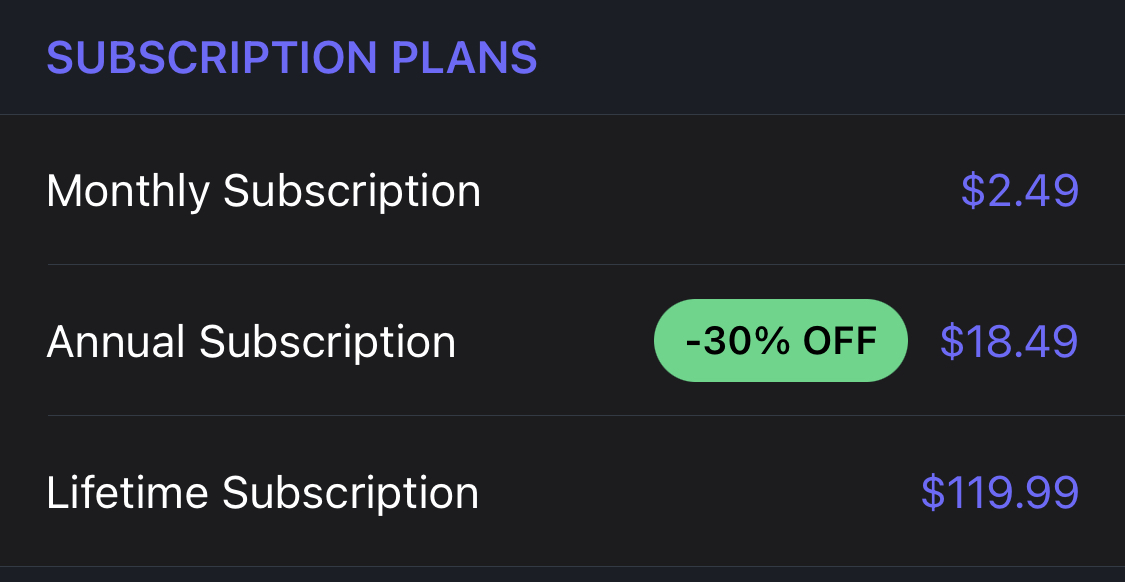
\includegraphics[width={0.7\linewidth}]{img/envision_app_price.jpeg}
\end{center}

Envision also has a pair of wearable glasses, built on top of the Google Glasses platform. All the features on the app are accessible with the glasses as well, as well as one additional feature that enables a video call that broadcasts a direct feed from the glasses. It is not clear from their website which of these features can run offline and which ones run online, as the glasses are capable of both wifi and Bluetooth. It's obvious that the video calling feature would require a network connection, but text detection could be done both offline or online. Additionally, the purchase of the glasses comes with a lifetime subscription to the accompanying application for both iOS and Android.

Similar to the OrCam MyEye, Envision is a great product with some cutting-edge features that are undeniably very useful for the visually impaired demographic. However, it suffers a similar problem in that it is very expensive. As of August 8th, 2021, the base model for Envision is listed as 3268.91 pounds, which is 5696.87 CAD.

\subsubsection{Seeing AI}
Seeing AI is a free application on iOS built as a part of Microsoft's "AI for Good" initiative \cite{seeing-ai}. Seeing AI has a lot of the same features that OrCam MyEye and Envision have, such as real-time short text detection, document reading, barcodes, face recognition, scene description, currency detection, and color detection. Two features that Seeing AI has that we couldn't confirm if MyEye or Envision have is handwritten text detection and light detection. Light detection is a unique feature that plays a sound that indicates how much light the camera detects. 

Some of these features work offline using on-device processing, while others utilize Microsoft's Azure cloud services and require a network connection. The features that require a network connection are document scanning, face detection, scene description, and handwritten text. The rest work offline.

The amazing part about this application is that it is totally free. There is no subscription or additional features available at a price. We found various other applications on the app store that would do a subset of features offered by Seeing AI, but they were not free. As a result, Seeing AI is considered the gold standard application for the visually impaired, as it is totally free and has a rich feature set. The individual we spoke to from Lighthouse SF was very familiar with this app and reported using it regularly.

After trying out this application, we really started to question if making a pair of glasses is even the way to go. If the end goal is to make it as cheap and accessible as possible, it's hard to compete with a free app that can do so much. The key insight that made us realize an affordable pair of glasses is still worthwhile to develop is the fact that it can be used without having to pull out and unlock your phone. Let's consider a specific example of wanting to read the name on a postcard. With Seeing AI, you'd have to pull out your phone, unlock it, find and open the Seeing AI app, switch to the "instant text" mode, and then have it read out the text for you. This might not seem so bad, but this process can be cumbersome for somebody who is visually impaired. However, with our solution, it would only require you to look towards the text you are trying to read, press a button on the glasses, and then after a small wait, the text will be read to you. This is fewer steps and allows you to more quickly read text out in the world. With this insight, we decided to continue pursuing our proposed design solution, even knowing now that a free alternative does exist.

\subsubsection{Speechify}
Speechify is a desktop and mobile app that can turn various forms of text into audio \cite{speechify}. The app is built on the premise that listening to something is easier and faster than reading it. It is not specifically for any demographic, but it can be used by anyone who has reading difficulty due to things like ADHD, Dyslexia, or visual impairment. Many people who have no problem reading still use Speechify, as it can increase productivity to get through large pieces of text faster by listening to it at faster speeds. Speechify can read anything on the internet, files, or images. It comes with a free option but there are paid features available, such as different voices that sound less robotic. This app was brought to our attention by UW AccessAbility services, as one of the complaints of many OCR technologies is the voice sounds very robotic, and Speechify was praised for having options for more realistic voices.

\subsubsection{Be My Eyes}
Be My Eyes is a free app that allows blind and visually impaired people to connect with sighted volunteers through a video call \cite{be-my-eyes}. This allows a sighted individual to assist in a task that a visually impaired person is having trouble with. Signing up to be a volunteer is free, and Connor has been a volunteer on the app for some time and has picked up three calls in the past. Waleed signed up for the app early in the term but has yet to get a notification to pick up a call. We examined this app as a way to potentially have interactions with visually impaired people, and get some insight into the kind of tasks that they need assistance with. An example use case would be for navigating an outdoor park. A visually impaired user may be in search of a bench to sit at and is not sure where to go. They can place a call for assistance on the app and a sighted volunteer will pick up and through the mobile phone's camera, guide the user to a nearby bench to sit at.

A notable mention is another app called Aira, which is built on the same premise as Be My Eyes, but instead of connecting visually impaired users with sighted volunteers, Aira employs trained visual interpreters who pick up the call.

Internally, we had some discussion about enabling a video call through the camera on the glasses, similar to the Envision glasses. This is not a high priority for us at the moment, but due to the success and usefulness of services such as Be My Eyes and Aira, it is something we are open to investigating further if time permits.

\subsubsection{Summary and Key Takeaways}
Assistive devices for the visually impaired is a problem space that has existed for quite some time, and as such, many solutions and products are currently available. Products like the OrCam MyEye 2, Envision, and Seeing AI offer a rich feature set and try to cover as many use cases as possible. The common feature, and the first one that each solution talks about, is the ability to detect and read text using OCR technology. It is reasonable to conclude that this is the most useful feature present in these solutions, and likely the one that gets the most usage. Therefore, we are choosing to focus on OCR as our primary feature, and only once we have that down will we start to consider some of the other features.

Additionally, due to the existence of Seeing AI, we plan on focusing our user experience around the glasses as much as possible. While we do want our app to eventually work without the glasses as well, and the user can simply use their phone's camera, it is less important to us since this functionality is already covered and implemented very well by Seeing AI. Our goal is to push this problem space forward with something that isn't too similar with what already exists.

\subsection{Patent Surveys}
The breadth of existing products with the same functionality as our solution has required us to carefully consider patent law when planning the design of our project. Specifically, OrCam owns a variety of patents protecting both their hardware and software products \cite{orcam-patents}. As the MyEye 2 is the device that most closely resembles our solution, we used their patent list as a starting point for our research. Other products, such as EnVision and NuEyes, possess IP as well, although these patents are either pending \cite{envision-patent} or unrelated to our solution.

Conveniently, the reason OrCam products are so expensive is also the reason we can successfully avoid patent infringement in our design. OrCam's patents are entirely related to proprietary software \cite{orcam-software} and hardware \cite{orcam-hardware}. Because we are using prefabricated hardware in the form of the Raspberry Pi and existing machine-learning software frameworks, neither of these components infringes upon OrCam's patents. OrCam does have some specific patents related to using a wearable camera in combination with machine learning software to drive an assistive device, although crucially these patents universally discuss performing machine learning on-platform. By offloading our machine-learning inference tasks to another device (the iPhone and servers), rather than using a dedicated processing device, our solution exists outside of the intellectual property patented by OrCam.

There is a possible issue of patent infringement concerning the doctrine of equivalents \cite{doctrine-of-equivalents}. This doctrine is a common legal rule which states that a device that does not literally fall within the realm of a patent may still be infringing upon said patent if it performs an identical function. This principle is often a legal grey area, and disputes regarding it are typically settled through a patent lawyer. While not experts, we believe that our solution avoids the doctrine of equivalents. While the system as a whole does perform a similar function to the OrCam MyEye 2, the subsystems involved do not. The wearable hardware's only purpose is to transmit an image wirelessly to either a server or a paired mobile app. In turn, the mobile application/server's only responsibility is to perform optical character recognition on an image. This image can be transmitted from an external source, or possibly captured by the smartphone camera. As a result, the solution performs an arguably different function entirely to OrCam's product. One of the qualifiers for the doctrine of equivalents to come into effect is that a "person skilled in the art" should consider the device or process equivalent to the patent being infringed upon \cite{doctrine-of-equivalents}. We feel confident that the novel addition of performing machine-learning on a mobile device and servers significantly differentiates our solution from OrCam's.


\newpage
\section{Design Solution Summary}

\section{Design Verification/Validation Summary}


\section{Design for Safety}

\section{Design for Regulatory Requirements}

\section{Impact on Society and Environment}

\section{Design Project Management Summary}

\section{Conclusions and Recommendations for Future Work}

\section{Acknowledgements}

\newpage
\section{Appendix A - Design Solution Description}
\subsection{System Level Representation}

\begin{figure}[H]
\centering
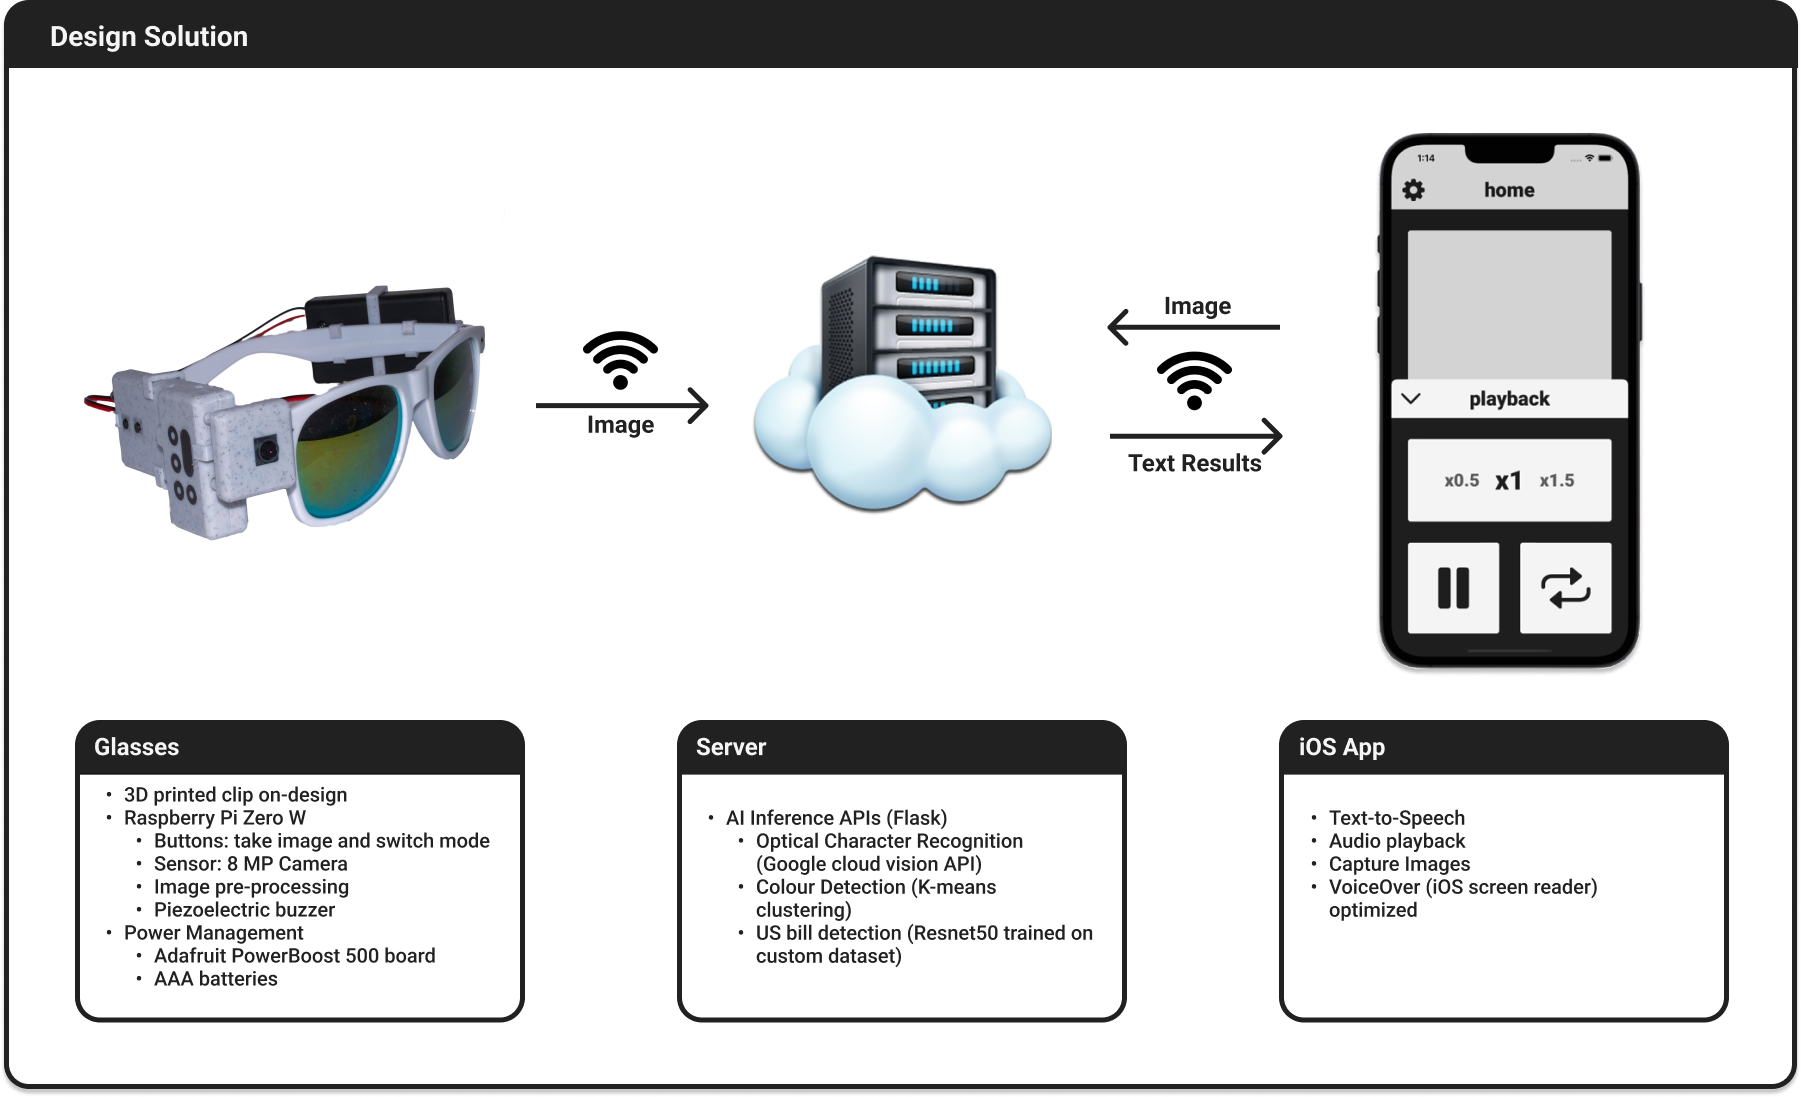
\includegraphics[scale=0.265]{img/system_diagram.png}
\caption{System design diagram}
\label{fig:system_diagram}
\end{figure}

Our design consists of 3 components: glasses, a server, and an iOS application. Figure \ref{fig:system_diagram} shows how these components interact with each other. The glasses send an image to the server, the server processes the image, and then the results are sent to the iOS app to be presented to the user through audio. The app is also capable of taking images and sending them to the server, and this allows the app to be used without the glasses.

Our original vision for this project was to avoid the need for an internet connection on the glasses and iOS device. Our goal was to do all of the computer vision processing on the iOS device and communicate information between the glasses and the iOS device using Bluetooth. However, we discovered Bluetooth limitations that make it impractical to reliably and quickly send an image over Bluetooth. See sections \ref{bluetooth} and \ref{apple-mfi} for more details.

\newpage
\subsection{Glasses}
\begin{center}
    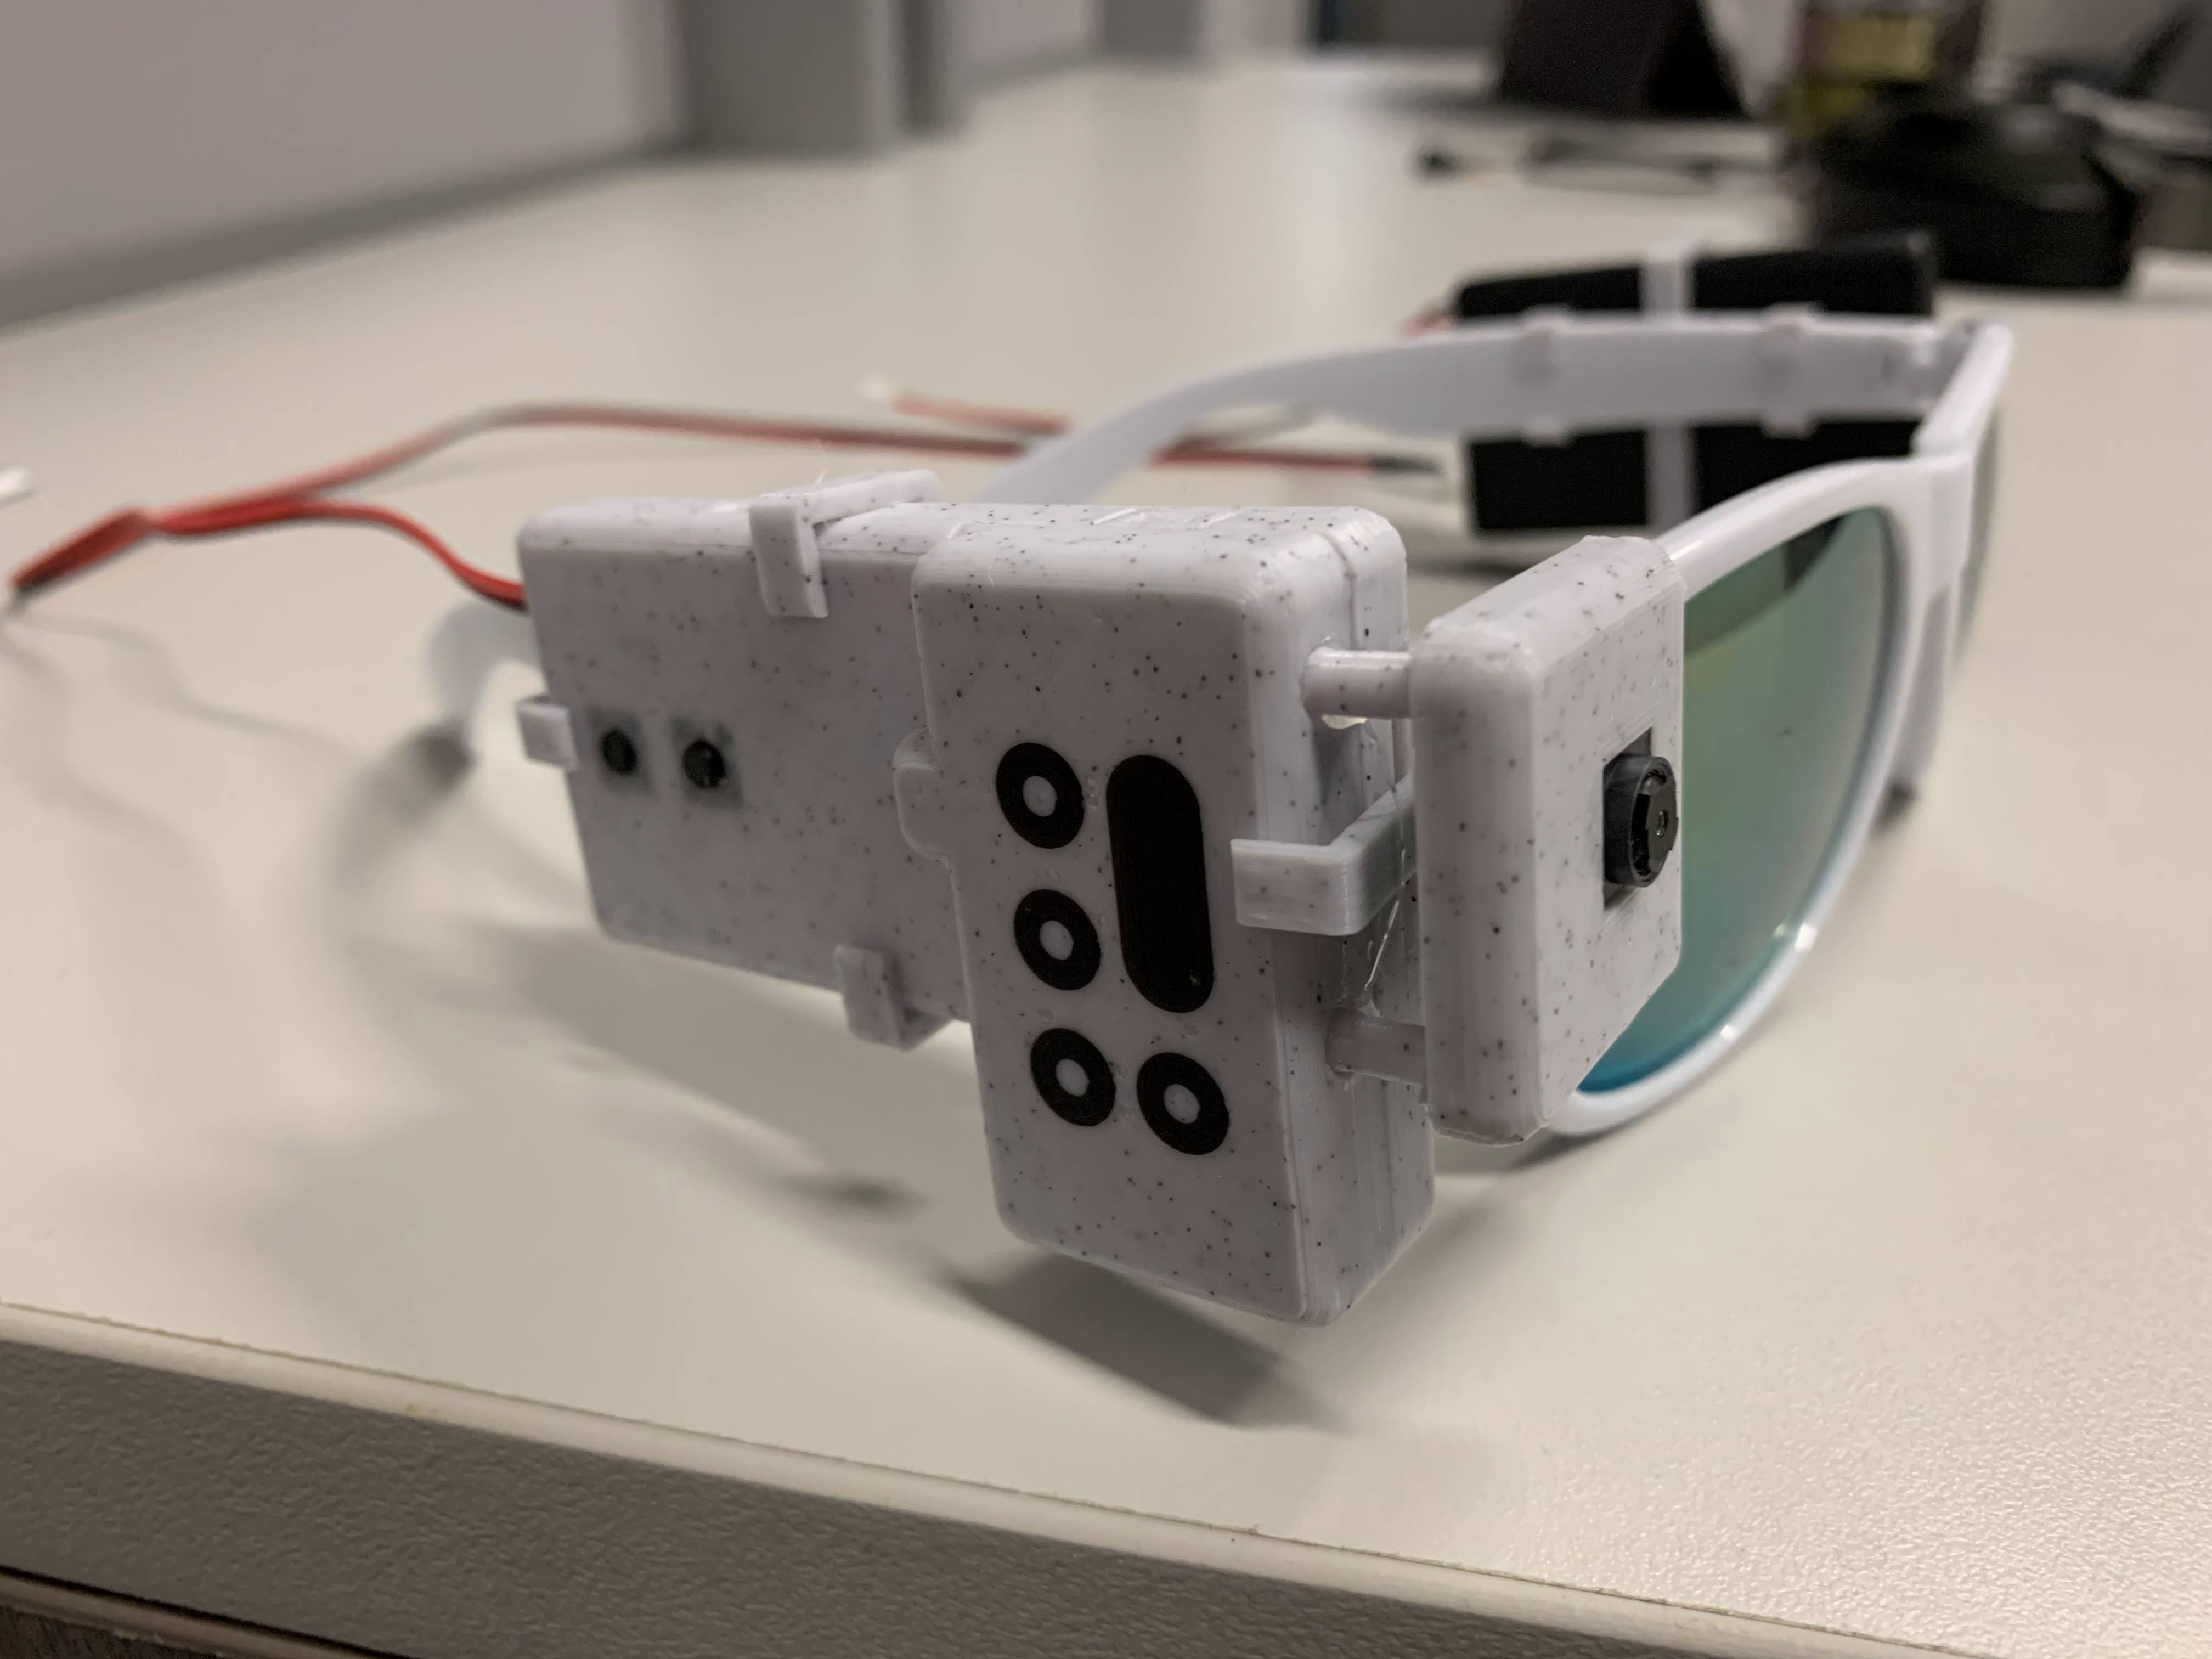
\includegraphics[width={0.3\linewidth}]{img/glasses/left.jpg}
    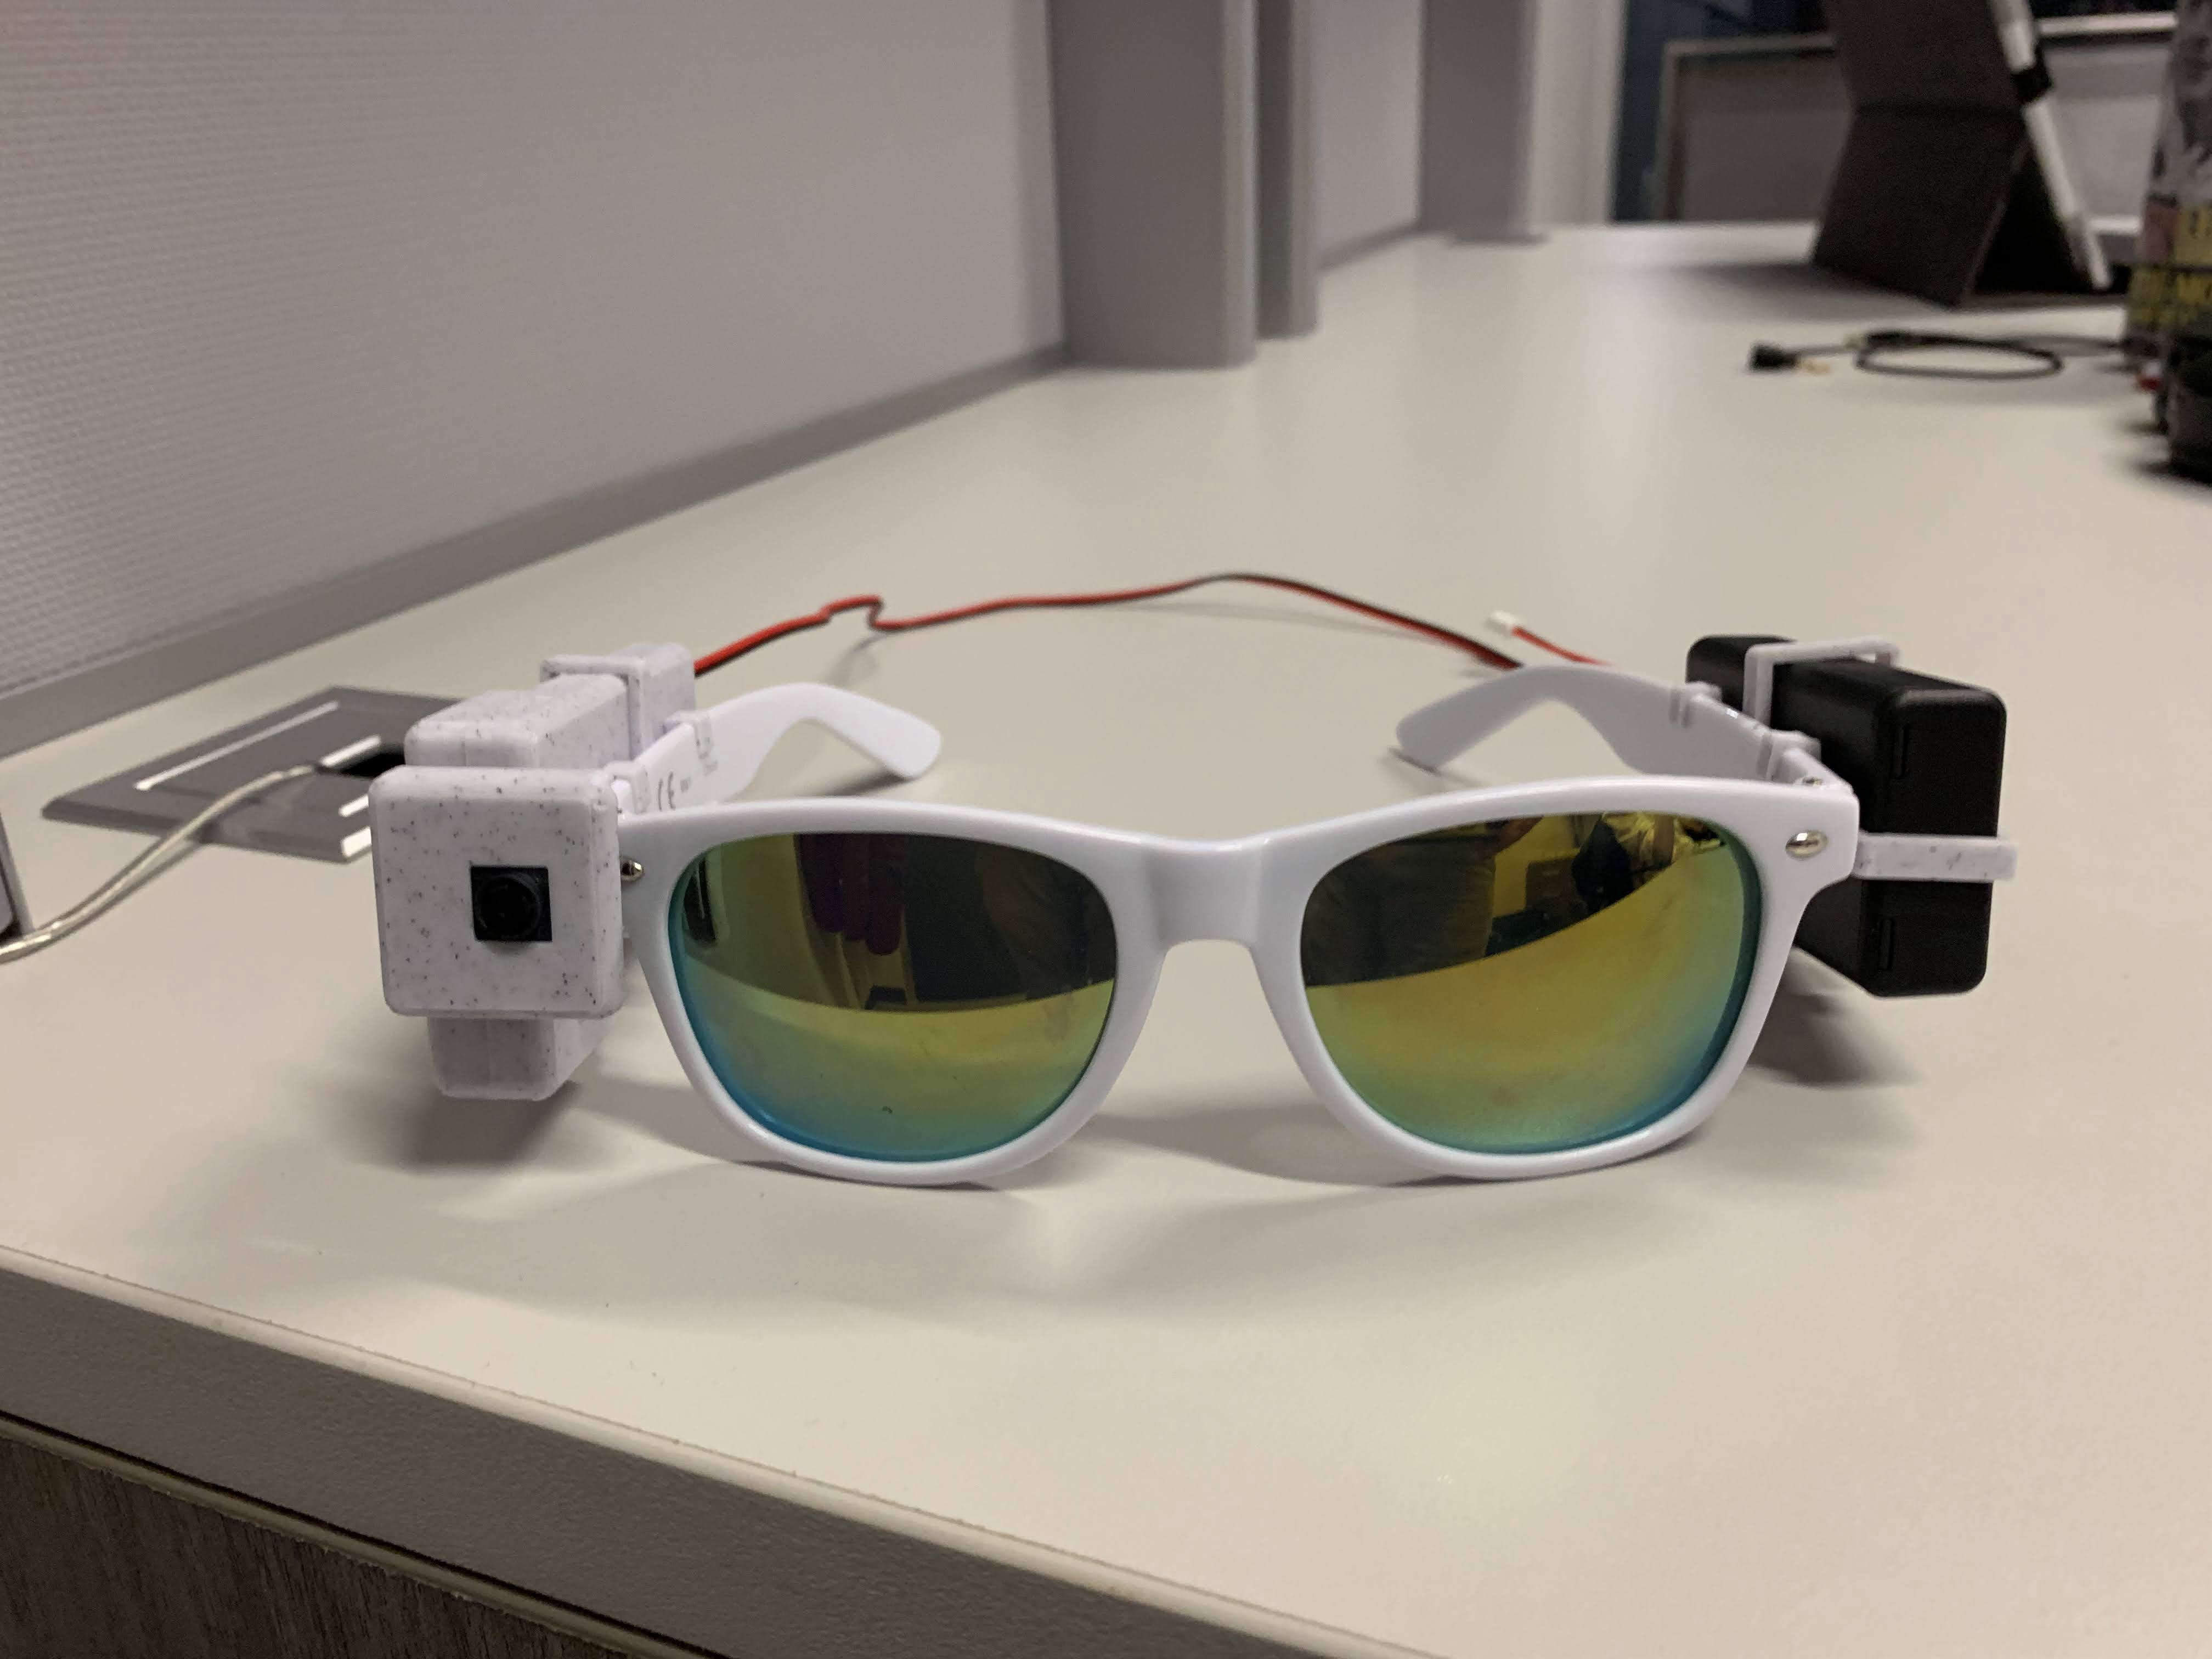
\includegraphics[width={0.3\linewidth}]{img/glasses/middle.jpg}
    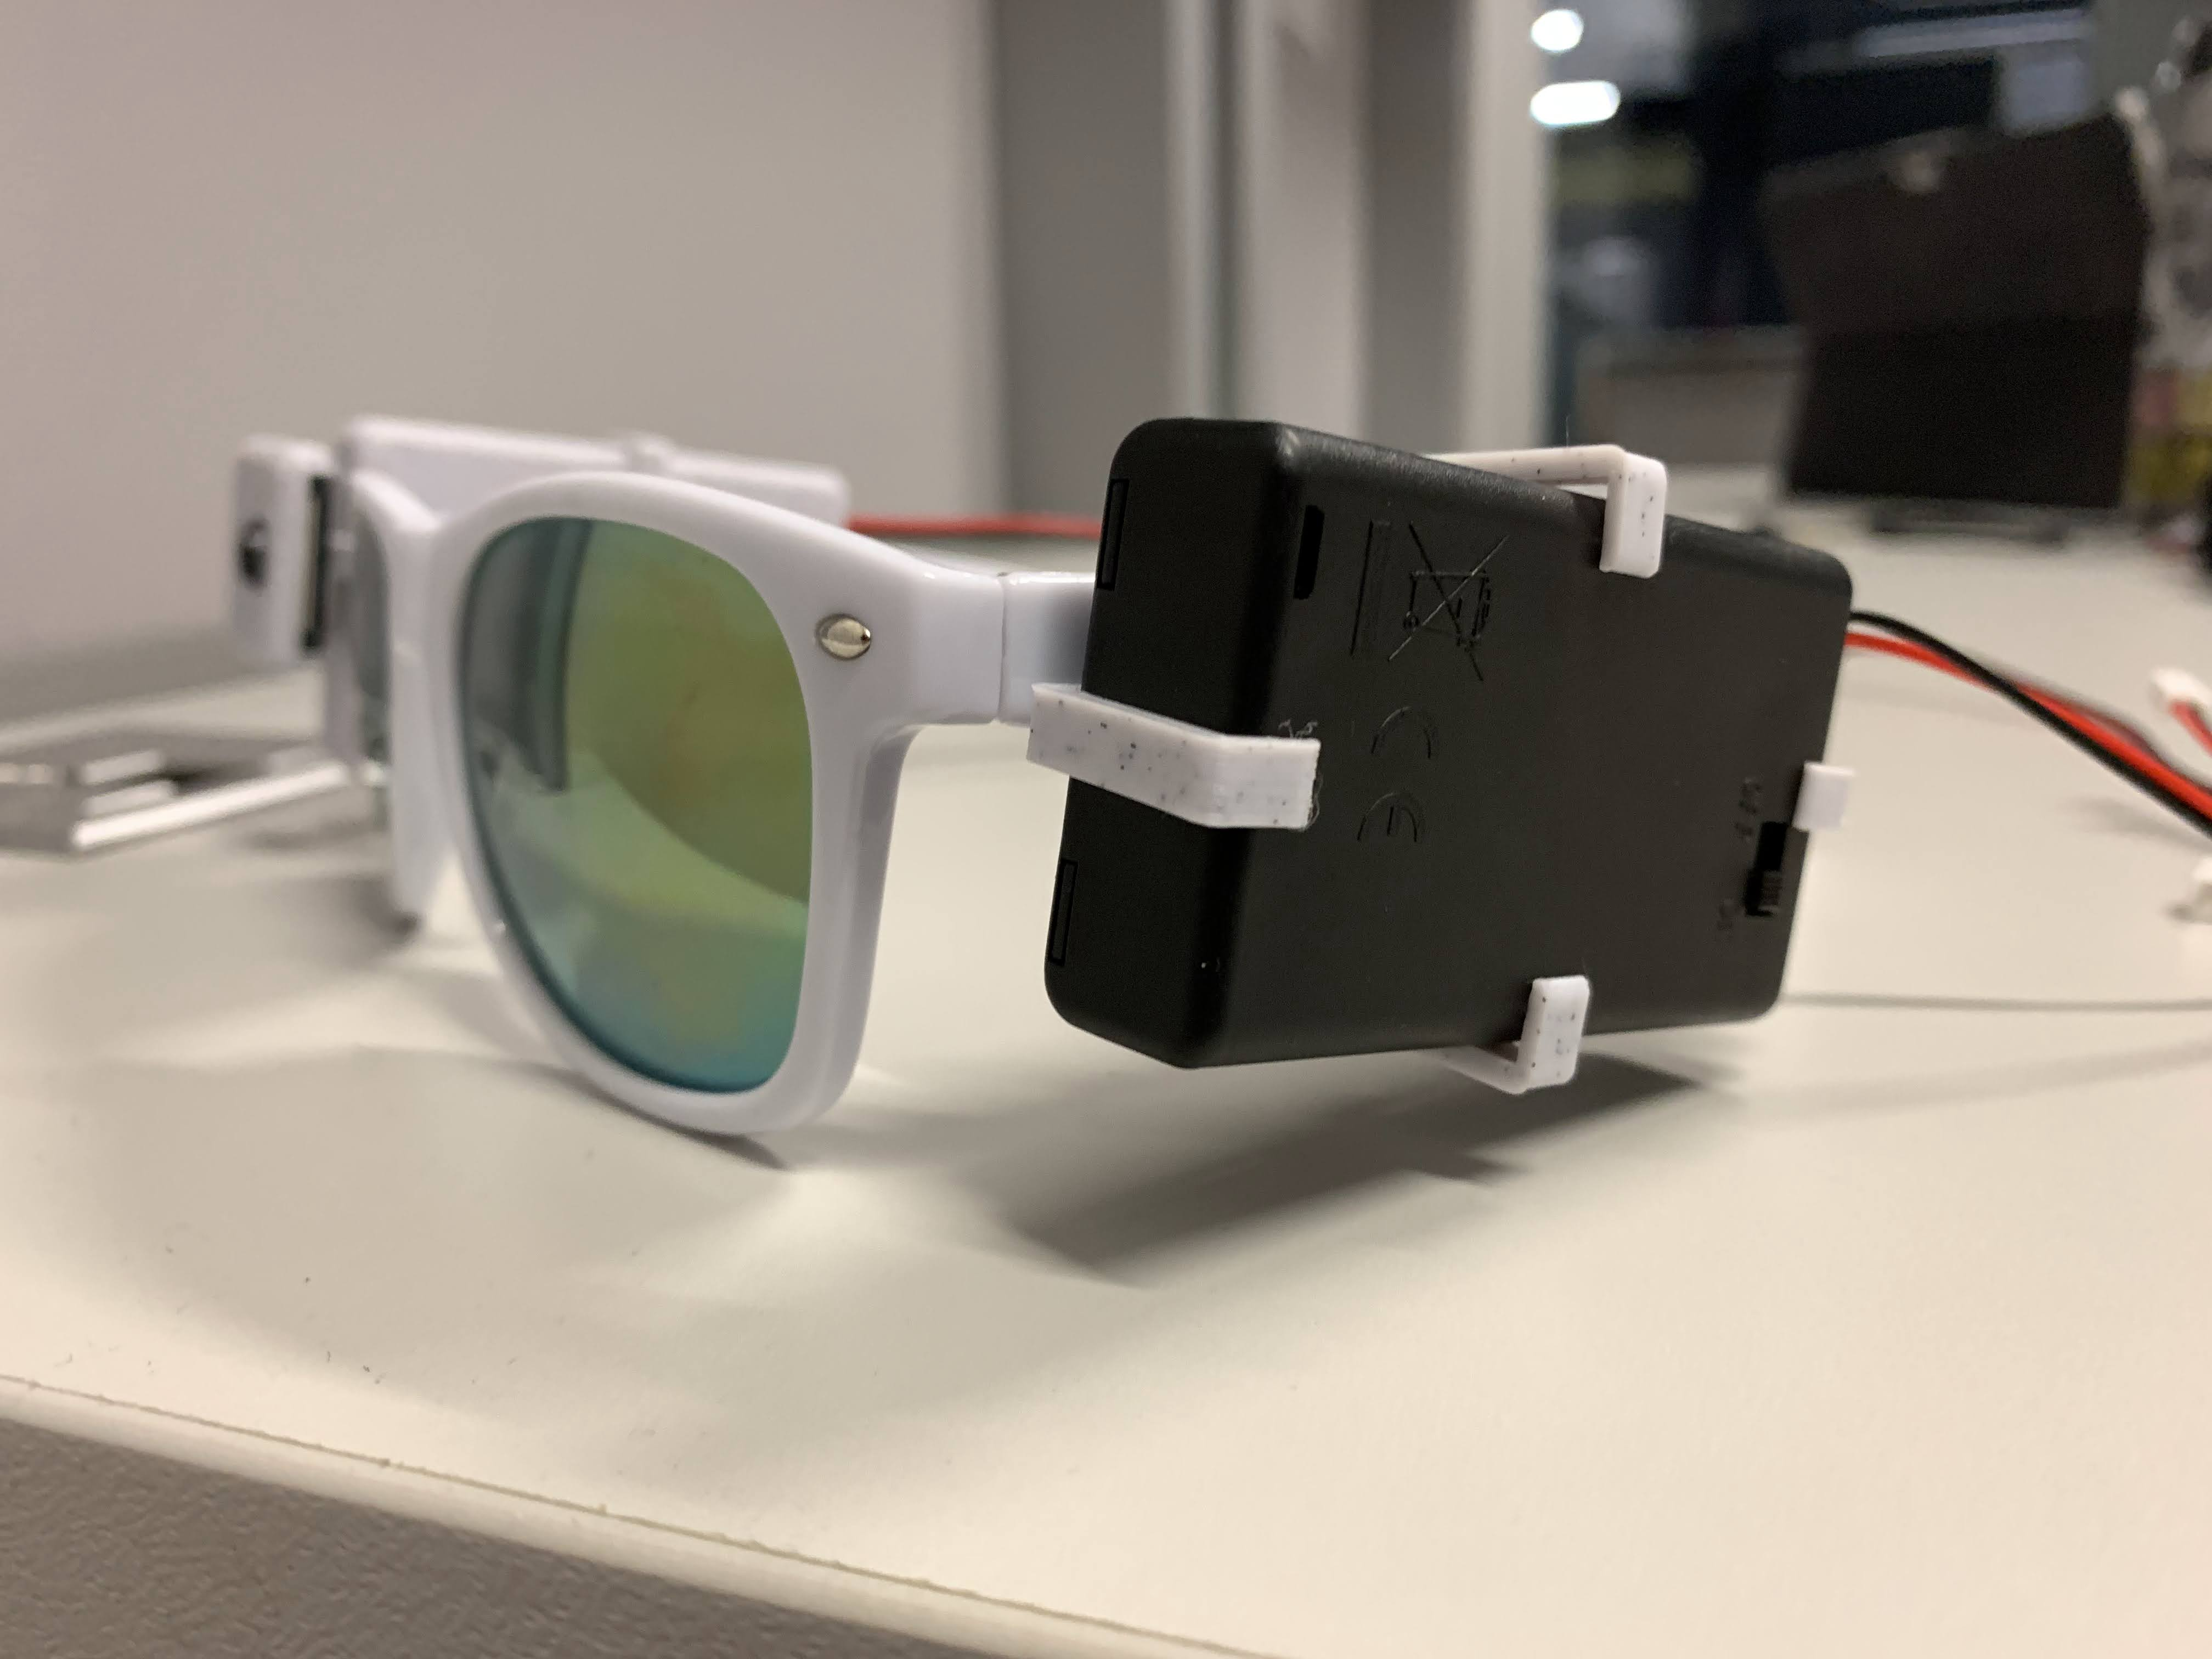
\includegraphics[width={0.3\linewidth}]{img/glasses/right.jpg}
\end{center}

A 3D printed clip-on design was used to allow flexibility since it can be attached to any pair of glasses. There are two pieces that attach to the glasses, the module on the right side is the compute unit, storing a Raspberry Pi Zero W, Adafruit PowerBoost 500, 8 MP Camera, 2 buttons, and a piezoelectric buzzer. The Raspberry Pi is responsible for all of the compute and managing the GPIO, the PowerBoost board is for power management, one button is to take a picture, another is to switch between different processing modes, and the piezoelectric buzzer is to communicate any errors or low battery warnings. The module on the left side is the power supply, which is a battery holder for 3 AAA batteries. There is a wire that goes between the 2 modules to connect the power supply, and this wire also doubles as a holder for the glasses in case the user wants to take it off their face and keep it around their neck. The great thing about this design is that the total cost of parts is less than 200 Canadian dollars, and the CAD files are provided by us so anybody can print the clip-on design using a 3D printer.

\subsection{Server}
\label{server}
The server is where all of the computer vision processing happens, and the results of the computation are sent back as a response and it can also be emitted on a socket, which the iOS app listens on so that it can receive the results in the event that the image was sent from the glasses. There are 3 features supported by the server: optical character recognition (OCR), colour detection, and money classification. The server is implemented in Flask, a micro web framework written in Python, and it was chosen since our computer vision code is implemented in Python, so having the server code in the same language makes it easier. There are 4 APIs exposed by the server:

\begin{itemize}
    \item \texttt{/ocr}: Performs optical character recognition.
    \item \texttt{/detect\_color}: Finds the top k colours in an image, with k being configurable.
    \item \texttt{/classify\_money}: Looks for all denominations of US bills. Also specifies when no bill is found in the image.
    \item \texttt{/socket\_emit}: Emits any string on a socket path. Used to communicate state changes from the glasses to the iOS app.
\end{itemize}

\subsubsection{Optical Character Recognition (OCR)}
Optical Character Recognition is generally a difficult task for computer vision systems. There are currently many existing solutions available to perform OCR. During the Spring 2021 term, different OCR libraries were tested and the best library was selected to be used in the project. Please refer to our Spring 2021 report for the details of the testing. In summary, we tested EasyOCR, PaddleOCR, Tesseract-OCR, and the Google Cloud Vision API, and found that the Google Cloud Vision API offered the best performance and the most features. This term, we further tested the google cloud vision API and became more confident in its performance and capabilities. One new feature we incorporated was language-specific text synthesis. We noticed the results from the Google API returned a language code for the text it finds, and we are able to forward this language code to the iOS app's speech synthesizer, and this way, it will speak the text in the locale of the language it is detected in. Google Cloud vision API currently supports 60 languages \cite{google-languages}, and while we didn't verify every single of them, we tried a subset of them with our iOS speech synthesis and it appeared to work well. Additionally, the Google vision API supports all three of our target modalities: text-in-the-wild, documents, and handwritten. See figure \ref{fig:google_vision_examples} below for example output from the Google APIs.

\begin{figure}[H]
\centering

\includegraphics[scale=0.5]{img/cv/ocr_text_in_the_wild.png}
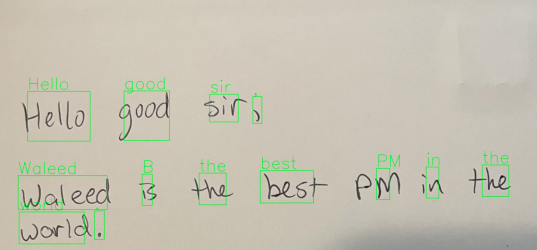
\includegraphics[scale=0.5]{img/cv/ocr_handwriting.png}
\caption{Examples of results from Google Cloud Vision API}
\label{fig:google_vision_examples}
\end{figure}

\subsubsection{Colour Detection}
Colour detection refers to identifying the most prevalent colours in an image. We got the idea to implement this since the feature exists in Seeing AI, and the individual we spoke with from Lighthouse SF mentioned she used this feature often to identify the colours of clothing, in order to decide what outfit to wear. We determined this would be a relatively straightforward algorithm to implement so we did it ourselves. Since the end goal is to report colours by name, and not the pixel values, we needed a database of colours with their associated RGB values to use as a reference. We used three such databases, which we referred to as small, medium, large, and they can be found
\href{https://github.com/vizia-fydp/server/tree/main/color_detection}{\color{blue}{here}}
 in our server repository. The small and medium databases are from \cite{color-small-medium}, and the large one is from \cite{color-large}. The small, medium and large databases have 17, 140, and 866 colours respectively. Note that we included HSV pixels for each colour as well as that is something we wanted to experiment with.

To implement this feature, we came up with two algorithms, described below:

\newpage
\begin{enumerate}
    \item For each pixel, find the euclidean distance to each colour in the database. The colour with the smallest euclidean distance is chosen as the best match for this pixel. Keep a count of which colours appear, and sort it by count, from highest to lowest count. Pick off the top K colours from this count.
    \item If K colours are desired, performs K-Means Clustering \cite{k-means-wikipedia, k-means-opencv} with 2*K clusters, pick out the top K clusters and calculate euclidean distance between the cluster mean and all colours in the database. Pick the colour from the database with the smallest euclidean distance as the match for that cluster.
\end{enumerate}

The equation for the euclidean distance can be seen in Equation \ref{eq:euclidean_dist}, where $d_i$ is the distance to the $i_{th}$ colour in the database. 

\begin{equation}
\label{eq:euclidean_dist}
d_i=\sqrt{(R - R_i)^2 + (G - G_i)^2 + (B - B_i)^2}
\end{equation}

Both algorithms were implemented and tested, and found that they produced similar results. However, algorithm 2 ran a little bit faster, even with optimizations made to algorithm 1. We kept code for both algorithms in the server code, but algorithm 2 is used due to its lower computational cost.

We choose to set K=3 to report the top 3 colours in the image as that seemed most appropriate, however, this parameter is easily configurable since the \texttt{/detect\_color} API takes K as an argument.

Figures \ref{fig:color-detection-output-1} - \ref{fig:color-detection-output-4} shows output of algorithm 2 using all three color databases, 6 k-means clusters, and the top 3 colour names.

\begin{figure}[H]
\centering
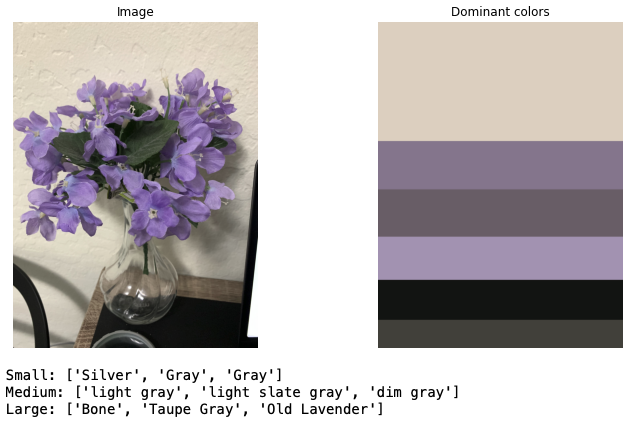
\includegraphics[scale=0.6]{img/cv/colour_detection/colour_detection_1.png}
\caption{Colour detection output}
\label{fig:color-detection-output-1}
\end{figure}

\begin{figure}[H]
\centering
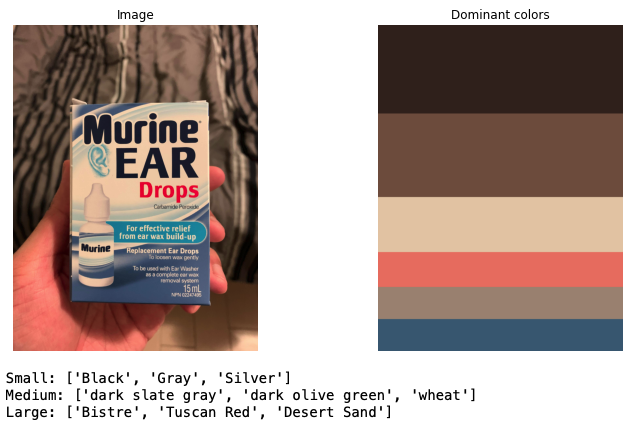
\includegraphics[scale=0.6]{img/cv/colour_detection/colour_detection_2.png}
\caption{Colour detection output}
\label{fig:color-detection-output-2}
\end{figure}

\begin{figure}[H]
\centering
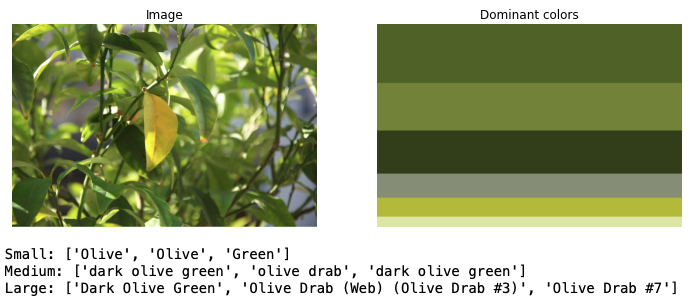
\includegraphics[scale=0.6]{img/cv/colour_detection/colour_detection_3.png}
\caption{Colour detection output}
\label{fig:color-detection-output-3}
\end{figure}


\begin{figure}[H]
\centering
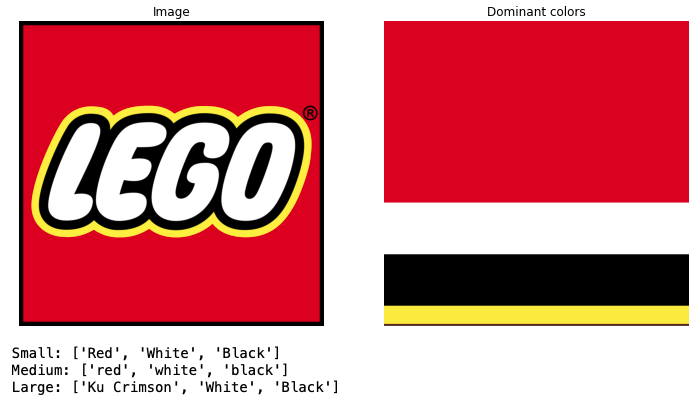
\includegraphics[scale=0.6]{img/cv/colour_detection/colour_detection_4.png}
\caption{Colour detection output}
\label{fig:color-detection-output-4}
\end{figure}

The small database isn't descriptive enough, the medium database has trouble with some real-world images, particularly in poor lighting conditions, and the large database is a little too descriptive, some of the colours sound confusing even to sighted individuals. We ended up choosing the medium database to use in production, as it works well as long as the lighting conditions are acceptable, so we can suggest to the user to use the flash on the phone when taking images.


\subsubsection{Money Classification}

\subsection{iOS App}

\newpage
\section{Appendix B - Verification and Validation Data}
\subsection{Bluetooth}
\label{bluetooth}
We had initially planned to use a Bluetooth Low Energy (BLE) connection to facilitate image transferring between the Raspberry Pi and the user's iOS device. We based this requirement around Apple's CoreBluetooth framework, and their restrictions on the amount of background processing iOS applications can perform. iOS has extremely aggressive memory and power management systems, which put apps into a suspended state when not in the foreground (i.e. when not open on the user's screen). Apple allows applications to request permission to perform background tasks, with certain limitations. One such permission is the ability to monitor communications from a paired BLE peripheral and act upon incoming data \cite{apple-bluetooth}. Once an incoming BLE packet destined for an application is detected, iOS provides a 15-30 second window for said application to complete any tasks it needs to do to react to this data before putting them back into a suspended state automatically.

We had planned to compress an image into JPEG format on the Raspberry Pi, then send a BLE notification to the iOS device that a new image was available for processing. The iOS device would then wake up the background application and pass along the BLE packet. The iPhone could then connect to the Raspberry Pi and retrieve the image. However, we discovered that BLE's extremely lightweight nature makes it impractical for transmitting large files (such as an image). The Raspberry Pi uses a Bluetooth 4.1 chip \cite{raspi-hardware}, which imposes a limit on the size of the data field in a transmitted BLE packet. The iPhone has a Bluetooth 4.2 chip \cite{iphone-hardware} which is capable of communicating with the Raspberry Pi's older chip, but is rate limited by the Pi's hardware. The maximum size of a data field in a packet sent between the two devices is therefore 27 bytes, although 4 of these bytes are used to store an offset (so that files larger than 27 bytes can be sent using consecutive packets. Additionally, iOS allows a maximum of 4 packets to be exchanged before a new BLE connection needs to be made. The BLE protocol also mandates a connection interval, which varies by device but is set to 15ms on all devices running iOS 11 or later \cite{apple-bluetooth}. This means that it would take almost a minute to transmit the smallest photo we could reasonably perform OCR on. This falls outside the window that iOS provides for a device to perform processing, before the application even receives the image.

Our workaround for this Bluetooth limitation was to drop the offline requirement and introduce a server between the glasses and iOS app that would be responsible for all the image processing and computer vision. See section \ref{server} for a detailed overview of the server.

A next step to bring our design closer to a final product would be to take advantage of the Apple MFi program \cite{apple-mfi}. This would allow us to remove the need for the server and honour our original requirement of having the glasses and iOS app work without a network connection. See section \ref{apple-mfi} for more.

\subsection{Apple MFi}
\label{apple-mfi}
Bluetooth Classic is a different version of Bluetooth which supports much higher throughput; BT Classic connections are two-way, continuous data streams up to 2.1Mbps \cite{bluetooth-classic}. iOS supports this version of Bluetooth, although it is restricted to embedded chips with Apple's MFi (Made For iPod) certification \cite{apple-mfi}. Using Bluetooth Classic would provide the data transfer speeds needed to send an image quickly enough to provide a good user experience, although the ability to perform background processing is restricted to BLE devices. Nevertheless, this would enable us to perform OCR on a piece of text and read it back while the user is offline. In our final product, we would apply for an Apple MFi certification in order to unlock the full potential of Bluetooth on iPhone.

\newpage
\section{Appendix C - Design Project Management Data}


\section{Appendix D - Knowledge Application}

\section{Exhibits}
\subsection{Promotional Video}
\subsection{Symposium Poster}
\subsection{GitHub}


\newpage
% REFERENCES
\begin{thebibliography}{9}
\bibitem{orbis-global-blind-data}
“Number of blind people set to triple by 2050” Orbis, 09-Feb-2021. [Online]. Available: https://can.orbis.org/en/news/2017/number-of-blind-people-set-to-triple-by-2050-1. [Accessed: 02-Aug-2021]. 

\bibitem{cnib-blind-data}
“Blindness in Canada” CNIB. [Online]. Available: https://cnib.ca/en/sight-loss-info/blindness/blindness-canada?region=on. [Accessed: 02-Aug-2021]. 

\bibitem{nfb-blind-data}
“Blindness Statistics” NFB, Jan-2019. [Online]. Available: https://nfb.org/resources/blindness-statistics. [Accessed: 02-Aug-2021]. 

\bibitem{lighthouse-sf-info-page}
“What does ‘blind’ really mean?” LightHouse for the Blind and Visually Impaired, 28-Jan-2019. [Online]. Available: https://lighthouse-sf.org/about/getting-started/. [Accessed: 02-Aug-2021]. 

\bibitem{WHO-blindness}
“Vision impairment and blindness” World Health Organization. [Online]. Available: https://www.who.int/news-room/fact-sheets/detail/blindness-and-visual-impairment. [Accessed: 02-Aug-2021]. 

\bibitem{lighthouse-sf-homepage}
LightHouse for the Blind and Visually Impaired, 22-Aug-2019. [Online]. Available: https://lighthouse-sf.org/. [Accessed: 02-Aug-2021].

\bibitem{uw-accessability}
AccessAbility Services, 08-Jul-2021. [Online]. Available: https://uwaterloo.ca/accessability-services/. [Accessed: 03-Aug-2021]. 

\bibitem{jaws-software}
“Jaws®” Freedom Scientific. [Online]. Available: https://www.freedomscientific.com/products/
software/jaws/. [Accessed: 03-Aug-2021].

\bibitem{kurzweil}
K. Education, Assistive learning technologies \& literacy software from KURZWEIL Education. [Online]. Available: https://www.kurzweiledu.com/default.html. [Accessed: 03-Aug-2021]. 

\bibitem{read-and-write}
“Read \& write for education - reading, literacy \& assistive software” Texthelp. [Online]. Available: https://www.texthelp.com/en-gb/products/read-and-write-education/. [Accessed: 03-Aug-2021]. 

\bibitem{speechify}
Speechify. [Online]. Available: https://speechify.com/. [Accessed: 03-Aug-2021]. 

\bibitem{clickup}
“ClickUp™ | one app to replace them all.” [Online]. Available: https://clickup.com/. [Accessed: 07-Aug-2021]. 

\bibitem{orcam}
OrCam MyEye 2.0. [Online]. Available: https://www.orcam.com/en/myeye2/. [Accessed: 08-Aug-2021].

\bibitem{orcam-price}
B. Holton, “MyReader and MyEye from OrCam: Text and item recognition at the touch of a finger,” The American Foundation for the Blind. [Online]. Available: https://www.afb.org/aw/18/2/15244. [Accessed: 08-Aug-2021]. 

\bibitem{orcam-amazon}
“OrCam MyEye Pro ,” Amazon.ca: Electronics. [Online]. Available: https://www.amazon.ca/OrCam-Inc-MyEye-2/dp/B07H31SBMW. [Accessed: 08-Aug-2021].

\bibitem{WHO-assistive}
“Assistive technology,” World Health Organization. [Online]. Available: https://www.who.int/news-room/fact-sheets/detail/assistive-technology. [Accessed: 08-Aug-2021]. 

\bibitem{envision}
Envision. [Online]. Available: https://www.letsenvision.com/. [Accessed: 08-Aug-2021].

\bibitem{seeing-ai}
Seeing AI App from Microsoft. [Online]. Available: https://www.microsoft.com/en-us/ai/seeing-ai. [Accessed: 08-Aug-2021]. 

\bibitem{speechify}
Speechify. [Online]. Available: https://speechify.com/. [Accessed: 08-Aug-2021]. 

\bibitem{be-my-eyes}
Be My Eyes - See the world together. [Online]. Available: https://www.bemyeyes.com/. [Accessed: 08-Aug-2021]. 

\bibitem{tesseract-github}
“Tesseract-Ocr/Tesseract: Tesseract open source ocr engine (main repository),” GitHub. [Online]. Available: https://github.com/tesseract-ocr/tesseract. [Accessed: 09-Aug-2021]. 

\bibitem{apple-speech-synthesis}
“Speech Synthesis,” Apple Developer Documentation. [Online]. Available: https://developer.apple.com/documentation/avfoundation/speech\_synthesis. [Accessed: 09-Aug-2021]. 

\bibitem{tesseract-improve-quality}
“Improving the quality of the output,” tessdoc. [Online]. Available: https://tesseract-ocr.github.io/tessdoc/ImproveQuality.html. [Accessed: 09-Aug-2021]. 

\bibitem{apple-mfi}
“Create innovative Accessories,” MFi Program. [Online]. Available: https://mfi.apple.com/. [Accessed: 10-Aug-2021]. 

\bibitem{apple-wac}
“Wireless Accessory Configuration Entitlement,” Apple Developer Documentation. [Online]. Available: https://developer.apple.com/documentation/bundleresources/entitlements/com\_apple\_external-accessory\_wireless-configuration. [Accessed: 10-Aug-2021]. 

\bibitem{rpi-zero-w}
“Raspberry Pi Zero W,” Raspberry Pi. [Online]. Available: https://www.raspberrypi.org/products/raspberry-pi-zero-w/. [Accessed: 10-Aug-2021]. 

\bibitem{rpi-camera}
“Camera Module 2,” Raspberry Pi. [Online]. Available: https://www.raspberrypi.org/products/camera-module-v2/. [Accessed: 10-Aug-2021]. 

\bibitem{wer-metric}
K. Leung, “Evaluate ocr output quality with character error rate (cer) and word error rate (wer),” Medium, 27-Jul-2021. [Online]. Available: https://towardsdatascience.com/evaluating-ocr-output-quality-with-character-error-rate-cer-and-word-error-rate-wer-853175297510. [Accessed: 10-Aug-2021].

\bibitem{levenshtein-dist}
“Levenshtein distance,” Wikipedia, 09-Mar-2021. [Online]. Available: https://en.wikipedia.org/wiki/Levenshtein\_distance. [Accessed: 10-Aug-2021].

\bibitem{scene-text-rec}
Y. Cao, S. Ma, and H. Pan, “FDTA: Fully CONVOLUTIONAL Scene text detection with TEXT ATTENTION,” IEEE Access, vol. 8, pp. 155441–155449, 2020.

\bibitem{iou-object-detection}
A. Rosebrock, “Intersection over Union (iou) for object detection,” PyImageSearch, 01-Jul-2021. [Online]. Available: https://www.pyimagesearch.com/2016/11/07/intersection-over-union-iou-for-object-detection. [Accessed: 10-Aug-2021].

\bibitem{paddle-ocr}
PaddlePaddle, “PaddlePaddle/PaddleOCR: Awesome Multilingual OCR toolkits based on PaddlePaddle (practical ultra lightweight OCR system, support 80+ Languages recognition, provide data annotation and synthesis tools, support training and deployment among server, mobile, embedded and Iot devices),” GitHub. [Online]. Available: https://github.com/PaddlePaddle/PaddleOCR. [Accessed: 10-Aug-2021].

\bibitem{easy-ocr}
JaidedAI, “JaidedAI/EasyOCR: Ready-to-use OCR with 80+ supported languages and all popular writing scripts including Latin, Chinese, Arabic, Devanagari, Cyrillic and etc.,” GitHub. [Online]. Available: https://github.com/JaidedAI/EasyOCR. [Accessed: 10-Aug-2021].

\bibitem{orcam-patents}
https://www.orcam.com/en/patents/

\bibitem{envision-patent}
https://patents.google.com/patent/US9805619B2/en

\bibitem{orcam-hardware}
https://patents.google.com/patent/US8902303B2/en

\bibitem{orcam-software}
https://patents.justia.com/patent/9911361

\bibitem{doctrine-of-equivalents}
“Doctrine of Equivalents”, Wikipedia, 02-Jun-2021. [Online]. Available: https://en.wikipedia.org/wiki/Doctrine\_of\_equivalents. [Accessed: 09-Aug-2021].

\bibitem{pipeda}
https://www.priv.gc.ca/en/privacy-topics/privacy-laws-in-canada/the-personal-information-protection-and-electronic-documents-act-pipeda/pipeda\_brief/

\bibitem{ewaste}
"What Are The Right Electronic Waste Disposal Methods?", Dawn DeVroom, 30-Apr-2019. [Online]. Available: https://blog.idrenvironmental.com/what-are-the-right-electronic-waste-disposal-methods. [Accessed: 9-Aug-2021]

\bibitem{neural-efficiency}
“Apple A11”, Wikipedia, 02-Jun-2021. [Online]. Available:
https://en.wikipedia.org/wiki/Apple\_A11. [Accessed: 9-Aug-2021].

\bibitem{iphone-recycle}
https://www.apple.com/ca/environment/

\bibitem{apple-bluetooth}
“Core Bluetooth”, Apple Developer Documentation. [Online]. Available: https://developer.apple.com/documentation/corebluetooth. [Accessed: 09-Aug-2021]. 

\bibitem{raspi-hardware}
https://www.raspberrypi.org/products/raspberry-pi-zero-w/

\bibitem{iphone-hardware}
“iPhone X Specifications”, Apple. [Online]. Available: https://support.apple.com/kb/sp770?locale=en\_CA. [Accessed: 09-Aug-2021]. 

\bibitem{bluetooth-classic}
"Bluetooth Classic vs Bluetooth Low Energy (BLE) on Android", D. Kliszowki, A. Vlasov. [Online]. Available: https://www.thedroidsonroids.com/blog/bluetooth-classic-vs-bluetooth-low-energy-ble. [Accessed: 09-Aug-2021].

\bibitem{resnet}
Singhal, G. (2020, May 5). Gaurav Singhal. Pluralsight. Retrieved December 4, 2021, from https://www.pluralsight.com/guides/introduction-to-resnet.

\bibitem{google-languages}
“OCR language support | cloud vision API |; google cloud,” Google. [Online]. Available: https://cloud.google.com/vision/docs/languages. [Accessed: 03-Apr-2022]. 

\bibitem{color-small-medium}
“RGB color codes chart - RapidTables.com.” [Online]. Available: https://www.rapidtables.com/web/color/RGB\_Color.html. [Accessed: 06-Apr-2022]. 

\bibitem{color-large}
Codebrainz, “Color-names/colors.csv at master · codebrainz/color-names,” GitHub, 01-Jul-2012. [Online]. Available: https://github.com/codebrainz/color-names/blob/master/output/colors.csv. [Accessed: 06-Apr-2022]. 

\bibitem{k-means-wikipedia}
“K-means clustering,” Wikipedia, 20-Mar-2022. [Online]. Available: https://en.wikipedia.org/wiki/K-means\_clustering. [Accessed: 05-Apr-2022].

\bibitem{k-means-opencv}
“K-means clustering in opencv,” OpenCV. [Online]. Available: https://docs.opencv.org/4.x/d1/d5c/tutorial\_py\_kmeans\_opencv.html. [Accessed: 05-Apr-2022]. 

\end{thebibliography}

\end{document}
